\section*{實驗目的:}
本實驗目的為使用ELISA分光光度計建立蛋白質濃度標準曲線,並測量未知蛋白質溶液濃度。預期蛋白質吸光值與蛋白質濃度呈線性,可根據已知濃度蛋白質溶液吸光值建立的迴歸直線與未知蛋白質溶液吸光值回推其濃度。

\section*{實驗步驟:}

\begin{enumerate}[label=\arabic*.]
  \item 實驗材料準備
  \begin{enumerate}[label=(\arabic*)]
    \item BSA胎牛血清蛋白,濃度為1 mg/ml,以1.5ml eppendorf裝取35\mul
    \item Bradford reagent,以離心管裝取2.5ml
    \item ddH2O,以1.5ml eppendorf裝取40ml
    \item 再取八支1.5ml eppendorf,其中六支標上組別1\~{}6,剩下兩支標示A、B
    \item unknown待測溶液
    \item 96孔盤,注意不要接觸盤底
    \item ELISA reader
    \item 微量吸管P2、P200、P1000 及 tip
    將1\~{}6及A、B eppendorf至於rack中,按照下表加入BSA及ddH2O。注意吸取微量體積時,tip不可沒入液面太深,避免取量誤差。
  \end{enumerate}
  
  \item 將1\~{}6及A、B eppendorf置於rack中,按照下表加入BSA及\ce{ddH2O}。{\color{red}注意}吸取微量體積時,tip不可沒入液面太深,避免取量誤差。

  \begin{table}[ht]
  \centering
  \begin{tabular}{ccc}
  \toprule
  管號&BSA \ce{(\mu l)}& \ce{ddH2O(\mu l)}\\
  \midrule
1&0&10\\
2&2&8\\
3&4&6\\
4&6&4\\
5&8&2\\
6&10&0\\
\midrule
A&5&5\\
B&10&0\\

\bottomrule
\end{tabular}\end{table}
\item 將Bradford reagent吸取300\mul 加入1\~{}6及A、B eppendorf。注意加入時不要碰到樣品,如此可重複使用tip。
\item 加入後,手指輕彈eppendorf底部,並靜置5分鐘。
\item 5分鐘後,自1\~{}6及A、B eppendorf吸取150\mul 樣品至96孔盤。
\item 96孔盤放入ELISA reader,待機器讀取後,紀錄讀值。

\end{enumerate}

\section*{實驗結果及討論:}
\subsection*{結果:}


\begin{table}[ht]
\caption{BAS吸光值回歸直線與未知BSA濃度} 
\setlength{\tabcolsep}{8mm}{
\begin{tabular}{llll}
\toprule
y=a+bx&第一次&第二次&第三次\\
\midrule
a&0.0334&0.0238&0.0300\\
b&0.0232&0.0224&0.0750\\
R$^2$&0.889&0.916&0.797\\
\midrule
A(mg/ml)&0.823&0.966&0.918\\
B(mg/ml)&0.799&0.884&0.867\\
平均&0.811&0.925&0.892\\
\bottomrule
\end{tabular}}
\end{table}


\subsection*{實驗數據:}


\begin{table}[ht]
  
  \label{tab:data}
  \caption{三次實驗實驗吸光值數據}
\begin{tabular}{lllllll}
\toprule
\multirow{2}*{BSA (mg)} & \multicolumn{2}{c}{第一次}  & \multicolumn{2}{c}{第二次}  & \multicolumn{2}{c}{第三次}  \\    
~ &OD$_{595nm}$&raw data&OD$_{595nm}$&raw data&OD$_{595nm}$&raw data\\
\midrule
0&0&0.122&0&0.119&0&0.731\\
2&0.107&0.229&0.091&0.21&0.116&0.847\\
4&0.12&0.242&0.102&0.221&0.29&1.021\\
6&0.199&0.321&0.177&0.296&0.799&1.53\\
8&0.244&0.366&0.229&0.348&0.517&1.248\\
10&0.227&0.349&0.216&0.335&0.707&1.438\\
\midrule
A(5\mul\ unknown)&0.144&0.266&0.132&0.251&0.374&1.105\\
B(10\mul\ unknown)&0.249&0.371&0.222&0.341&0.68&1.411\\
\bottomrule
      
  \end{tabular}
\end{table}





\subsection*{實驗作圖:}
  
\begin{figure}[H]
\centering
\begin{minipage}[b]{0.45\textwidth} %minipage寬
\centering
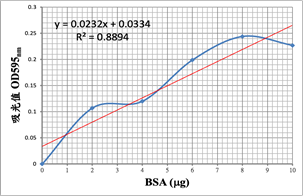
\includegraphics[width=.9\textwidth]{paste_src/2023-09-28-04-14-53.png}
\caption{第一次實驗迴歸直線}
\label{fig:1}
\end{minipage}
\begin{minipage}[b]{0.45\textwidth} %minipage宽
\centering
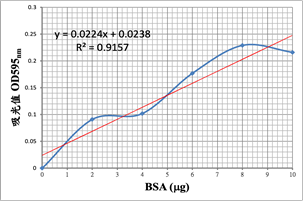
\includegraphics[width=.9\textwidth]{paste_src/2023-09-28-04-14-34.png}
\caption{第二次實驗迴歸直線}
\label{fig:2}
\end{minipage}
\end{figure}


\begin{figure}[H]\centering
\begin{minipage}[b]{0.4\textwidth} %minipage寬
\centering
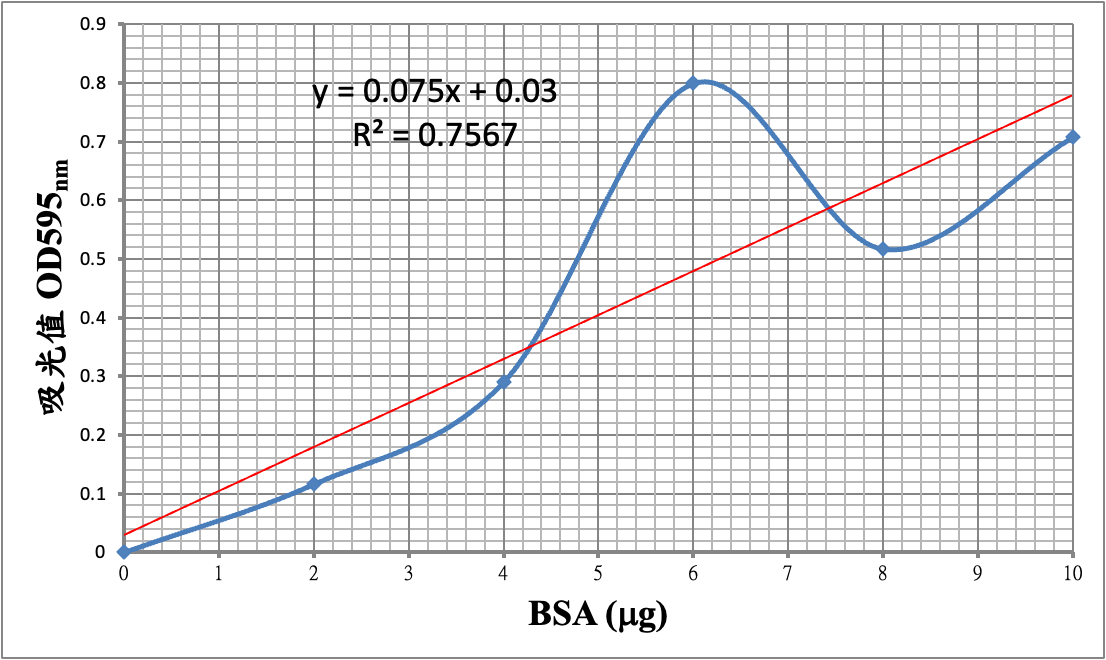
\includegraphics[width=1\textwidth]{paste_src/2023-09-28-17-19-36.png}
\caption{第三次實驗迴歸直線}
\label{}
\end{minipage}
\end{figure}

\subsection*{實驗討論:}

\begin{enumerate}[label=\arabic*.]
  \item 如果實驗上有誤差,可能造成的原因為何?
  \begin{enumerate}[label=(\arabic*)]
    \item 操作微量吸管技術不佳,在吸取2\~{}10\mul 時,可能將tip插入液面太深,使tip外部沾取過多樣品,使得後續濃度出現誤差。
    \item 機器量測問題,老師有提到我們使用的機器在過往觀察中有個傾向是會在第6個樣品的吸光值會降低。
    \item 染色時間問題,我們組一共做出兩個R平方值,使用同一台機器在不同時間讀取,推測,如果染劑應該能與蛋白質維持一段時間穩定結合,那也有可能是染劑老化,品質較差。
  \end{enumerate}

  \item 如何減少本次實驗所造成的誤差與錯誤?\\
  在其他組有做出R平方值高達0.98的情況下,我認為最主要還是自己操作微量吸管的技巧要再更加精進。
  \item 與本次實驗相關的其他方法或研究。

\end{enumerate}


\section*{參考資料:}
如果有使用到任何參考資料,請列出來源及出處。

*You can also write the report in English if you want/need to.
